\resizebox{\linewidth}{!}{
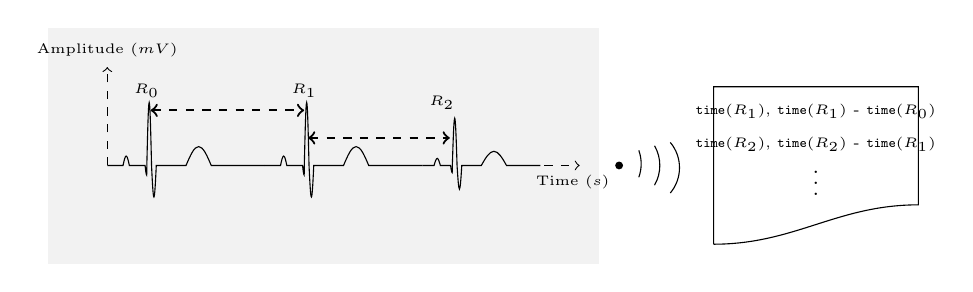
\begin{tikzpicture}
    % Colors definition
    \pgfdeclaredecoration{single pulse}{initial}{
    \state{initial}[width=\pgfdecoratedinputsegmentlength]
    {%
        % Initial Line
        \pgfpathlineto{\pgfpoint{0.1*\pgfdecoratedinputsegmentlength}{0mm}}%    
        % P Peak
        \pgfpathsine{\pgfpoint{0.2\pgfdecorationsegmentlength}{0.15\pgfdecorationsegmentamplitude}}%
        \pgfpathcosine{\pgfpoint{0.2\pgfdecorationsegmentlength}{-0.15\pgfdecorationsegmentamplitude}}%
        % P - Q Line
        \pgfpathlineto{\pgfpoint{0.6\pgfdecorationsegmentamplitude}{0mm}}%
        % Q Valley
        \pgfpathsine{\pgfpoint{0.1\pgfdecorationsegmentlength}{-0.15\pgfdecorationsegmentamplitude}}
        \pgfpathcosine{\pgfpoint{0.01\pgfdecorationsegmentlength}{0.15\pgfdecorationsegmentamplitude}}%
        % R Peak
        \pgfpathsine{\pgfpoint{0.15\pgfdecorationsegmentlength}{\pgfdecorationsegmentamplitude}}%
        \pgfpathcosine{\pgfpoint{0.15\pgfdecorationsegmentlength}{-\pgfdecorationsegmentamplitude}}%
        % S Valley
        \pgfpathsine{\pgfpoint{0.15\pgfdecorationsegmentlength}{-0.5\pgfdecorationsegmentamplitude}}
        \pgfpathcosine{\pgfpoint{0.15\pgfdecorationsegmentlength}{0.5\pgfdecorationsegmentamplitude}}%
        % S to T line
        \pgfpathlineto{\pgfpoint{1.25\pgfdecorationsegmentamplitude}{0mm}}%
        % T Peak
        \pgfpathsine{\pgfpoint{0.8\pgfdecorationsegmentlength}{0.3\pgfdecorationsegmentamplitude}}%
        \pgfpathcosine{\pgfpoint{0.8\pgfdecorationsegmentlength}{-0.3\pgfdecorationsegmentamplitude}}%
        % Last Line
        \pgfpathlineto{\pgfpointdecoratedinputsegmentlast}%
    }
    \state{final}{}%
    }

    \fill[gray!10] (-0.75, -1.25) rectangle (6.25, 1.75);
    %\node at (5.5, 1.5) {\textbf{\small{Sensor}}};

    \draw[->, dashed] (5.55,0) -- (6,0) node[pos=.8, anchor=north] {\tiny{Time ($s$)}};
    \draw[->, dashed] (0,0) -- (0,1.25) node[anchor=south] {\tiny{Amplitude ($mV$)}};
    \draw[decoration={single pulse,amplitude=8mm,segment length=2mm},decorate] (0,0) -- (2,0);
    \draw[decoration={single pulse,amplitude=8mm,segment length=2mm},decorate] (2,0) -- (4,0);
    \draw[decoration={single pulse,amplitude=6mm,segment length=2mm},decorate] (4,0) -- (5.5,0);
    \draw[<->, dashed, thick] (0.55, 0.7) -- (2.5, 0.7);
    \draw[<->, dashed, thick] (2.55, 0.35) -- (4.35, 0.35);
    \node[align=center] at (0.5, 0.95) {\tiny{$\text{R}_0$}};
    \node[align=center] at (2.5, 0.95) {\tiny{$\text{R}_1$}};
    \node[align=center] at (4.25, 0.8) {\tiny{$\text{R}_2$}};

    % Signal
    \fill[black] (6.5, 0) circle (0.05);
    \draw (6.75, -0.15) arc (-20:20:0.5);
    \draw (6.95, -0.25) arc (-30:30:0.5);
    \draw (7.15, -0.35) arc (-40:40:0.5);

    % Data file
    \draw (7.7, -1) -- (7.7, 1) -- (10.3,1) -- (10.3, -0.5) to[out=180, in=0] (7.7, -1);
    \node[align=center] at (9, 0.2) {\tiny{\texttt{time}$\left(\text{R}_1\right)$, \xspace\texttt{time}$\left(\text{R}_1\right)$ - \texttt{time}$\left(\text{R}_0\right)$} \\ \tiny{\texttt{time}$\left(\text{R}_2\right)$, \xspace\texttt{time}$\left(\text{R}_2\right)$ - \texttt{time}$\left(\text{R}_1\right)$} \\ \tiny{\textbf{$\vdots$}}};
%    % Main outline
%    %\draw[fill=green1] (0,0) rectangle (10, 1) node[pos=.5] {Privileged System Code, OS, VMM};
%    \draw[fill=gray!10] (0, 0) rectangle (10, 8.5);
%
%    % Unsecure Part
%    \node[align=center] at (2.25, 7.5) {\textbf{Untrusted Code}};
%    \draw[dashed, fill=white] (0.5, 0.5) rectangle (4, 7.0);
%    \node at (1.25, 1.25) {\includegraphics[width=25pt]{resources/img/hacker.png}};
%    \draw[->,thick, decorate,decoration={snake, post=lineto, post length=1mm}] (2.25, 6.5) -- (2.25, 5.75) node[pos=.3,anchor=west] {\blackcircled{1}};
%    \node[align=center] at (2.25, 5.5) {\texttt{Create Enclave}};
%    \draw[->,thick, decorate,decoration={snake, post=lineto, post length=1mm}] (2.25, 5) -- (2.25, 4) node[pos=.5,anchor=west] {\blackcircled{2}};
%    \node[align=center] at (2.25, 3.5) {\texttt{Call Trusted} \\ \texttt{Function}};
%    \draw[->,thick, decorate,decoration={snake, post=lineto, post length=1mm}] (2.25, 3) -- (2.25, 2) node[pos=.3,anchor=west] {\blackcircled{7}};
%    \draw[->, very thick] (4, 5.25) -- (5.5, 5.25) node[pos=.5,anchor=south] {\circled{3}};
%
%    % Secure Part
%    \node[align=center] at (7.75, 7.5) {\textbf{Trusted Code}};
%    \draw[fill=white] (6, 0.5) rectangle (9.5, 7.0);
%    \node at (8.75, 1.25) {\includegraphics[width=25pt]{resources/img/intel-sgx.png}};
%    \node[align=center] at (5.55, 6.5) {\small{Call} \\ \small{Gate}};
%    \draw[fill=gray!80] (5.5, 5.5) rectangle (6, 6.0);
%    \draw[fill=gray!80] (5.5, 5.0) rectangle (6, 5.5);
%    \draw[fill=gray!80] (5.5, 4.5) rectangle (6, 5.0);
%    \draw[rounded corners, dashed] (6.5, 2.5) rectangle (9, 5.75);
%    \draw[->, very thick] (5.75, 5.25) -- (6.75, 5.25) node[pos=.5,anchor=south] {\blackcircled{4}};
%    \node[align=center] at (7.75, 5.25) {\texttt{Execute}};
%    \draw[->,thick, decorate,decoration={snake, post=lineto, post length=4mm}] (7.75, 5) -- (7.75, 3.25) node[pos=.5,anchor=west] {\circled{5}};
%    \node[align=center] at (7.75, 3) {\texttt{Return}};
%    \draw[->, very thick] (6.75, 3) -- (4, 3) node[pos=.6, anchor=south] {\circled{6}};
\end{tikzpicture}}
